
\section{Determining the spin mass}

Following the method in section~\ref{Sec:Exp:MeasuringSpinMass} we begin by taking a variety of spin masses using the cylindrical approximation. Figure~\ref{Fig:ResD:Band4SpinMassCylindrical} shows \ac{FFT} amplitudes for a portion of the $\alpha$ electron pocket taken over a range of angles towards the $[100]$ direction. The shaded areas are bound to the areas where we believe the amplitudes go to zero as defined by the overall shape of the curve and the splitting of the peaks. The upper panel shows the particular oscillation that most closely matches the zeros in the data as well as its upper and lower bounds to quantify the possible error. The lower panel shows the next and previous set of oscillations in order to demonstrate that the selected oscillation in the top panel is indeed the best fit. In the cylindrical case the best fit is given by \TODO{XXXXX} with an error of \TODO{XXXX}.
\begin{figure}[htbp]
    \begin{center}
        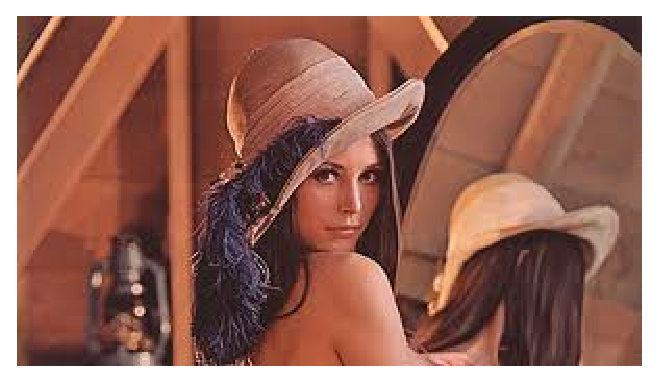
\includegraphics[scale=0.9]{Misc/TODO}
        \caption{Measured amplitude of \ac{FFT} peaks across a range of angles for the portion of data shown in the inset. Curves corresponding to the $A_S$ term calculated using the cylindrical apporximation are superimposed. Upper panel shows the best fitting data and its bounds, the lower portion shows fitting to the next oscillation along which clearly demonstrates the misalignment. Shaded areas are zones where we believe the spin zeros are located in the data.}
        \label{Fig:ResD:Band4SpinMassCylindrical}
    \end{center}
\end{figure}
We now contrast this with a spin mass determination using a band mass calculated from \ac{DFT}. Figure~\ref{Fig:ResD:DFTBandMassBand4} shows the band mass as calculated from the shifted \ac{DFT} energies for band 4. On the plot is an order 8 polynomial fit as well as the corresponding cylindrical approximation curve for comparison.
\begin{figure}[htbp]
    \begin{center}
        \includegraphics[scale=0.9]{Chapter-dHvABaFe2P2/Figures/Mass/DFTBandMassBand4/DFTBandMassBand4}
        \caption{Band masses calculated from \ac{DFT} of band 4 taken over a range of angles rotating towards the $[100]$ direction. A fit to and order 8 polynomial is shows as well as a comparitive fit suing the cylindrical approximation.}
        \label{Fig:ResD:DFTBandMassBand4}
    \end{center}
\end{figure}
Taking the polynomial from the fit to the \ac{DFT} band mass calulcations as the band mass for the inspection of the $A_S$ term, figure~\ref{Fig:ResD:SpinMassFromDFTBand4} shows the revised best fit. Now the fit values gives a spin mass of \TODO{XXXX} with an error pf \TODO{XXXX}.
\begin{figure}[htbp]
    \begin{center}
        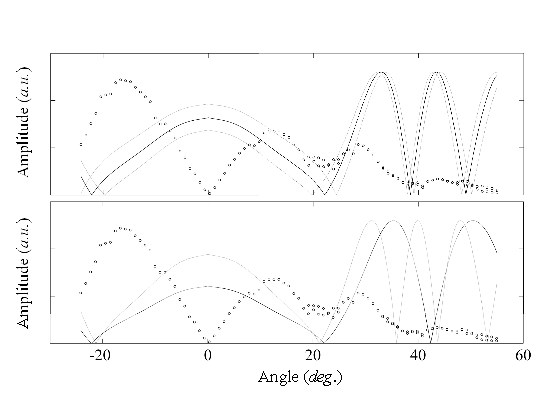
\includegraphics[scale=0.8]{Chapter-dHvABaFe2P2/Figures/Mass/SpinMassBand4/SpinMassBand4}
        \caption{Measured amplitude of \ac{FFT} peaks across a range of angles for the portion of data shown in the inset.  Curves corresponding to the $A_S$ term calculated using the cylindrical apporximation are superimposed. Upper panel shows the best fitting data and its bounds, the lower portion shows fitting to the next oscillation along which clearly demonstrates the misalignment. Shaded areas are zones where we believe the spin zeros are located in the data.}
        \label{Fig:ResD:SpinMassFromDFTBand4}
    \end{center}
\end{figure}
Given that a more accurate fit is obtained by using the \ac{DFT} calculated band masses, table~\ref{Table:ResD:SpinMassValues} shows more spin mass values calculated using this technique with the full graphs given in Appendix~\ref{Appendix:SpinMassPlots}.
\begin{table}
    \begin{center}
           \caption{Spin mass values calculated using inspection of measured data. Values calculated from \ac{DFT} were used for the band mass term.}
        \begin{tabular}[htbp]{ll}
\toprule
Band    &   $m^*_S$ \\
\midrule
\TODO{XXXX} & \TODO{XXXX} \\
\bottomrule
        \label{Table:ResD:SpinMassValues}
        \end{tabular}
    \end{center}
\end{table}
